\documentclass[12pt]{article}
\usepackage[table]{xcolor}
\usepackage[shortlabels]{enumitem}
\usepackage{tabularx,xltabular}
\usepackage{graphicx}
\usepackage{hyperref}
\usepackage{verbatim}
\usepackage{geometry}
\usepackage{ulem}
\usepackage[official]{eurosym}
\usepackage{tikz}
\usetikzlibrary{arrows,backgrounds,calc,decorations.markings,patterns,3d,positioning,fit,angles, quotes}
\usepackage{pgfplots}
\pgfplotsset{compat = newest}
\usetikzlibrary{fit}
\newcommand\addvmargin[1]{
\usetikzlibrary{arrows}
\node[fit=(current bounding box),inner ysep=#1,inner xsep=0]{};}
\usepackage{cancel}
\usepackage{fontspec}
\usepackage{array}  
\geometry{a4paper, top=2cm, left=2cm, right=2cm, bottom=2cm, headsep=1cm}
\usepackage{tabu}
\usepackage{pst-node}
\usepackage{colortbl}
\usepackage{array}
\usepackage{german}
\setlength\parindent{0pt}
\newcolumntype{?}{!{\vrule width 1pt}}
\usepackage{makecell}
\renewcommand{\arraystretch}{2.5}
\usepackage{pbox}
\usepackage{amssymb}
\usepackage{amsmath}
\usepackage{booktabs}
\newcolumntype{L}[1]{>{\raggedright\let\newline\\\arraybackslash\hspace{0pt}}m{#1}}
\newcolumntype{C}[1]{>{\centering\let\newline\\\arraybackslash\hspace{0pt}}m{#1}}
\newcolumntype{R}[1]{>{\raggedleft\let\newline\\\arraybackslash\hspace{0pt}}m{#1}}
\begin{document}
\rightline{Datum: 08.12.2023}
\centerline{{\Large Tägliche Übungen}} 
\vspace{1cm}
\noindent \\


\begin{xltabular}{\textwidth}{|C{0.75cm}|X|C{0.75cm}|X|}
\arrayrulecolor{black}\hline
a)&\pbox{5cm}{
Berechne den Flächeninhalt von:\\
\tikzstyle{background grid}=[draw, black!15,step=.5cm]
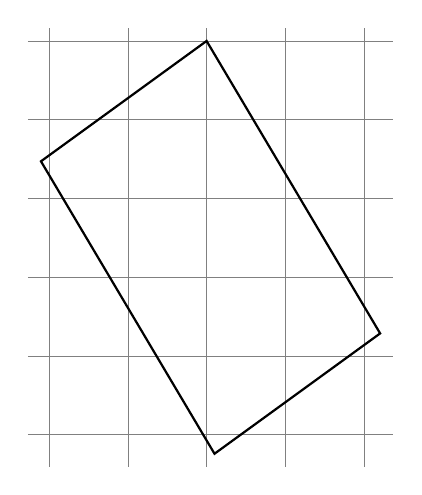
\begin{tikzpicture}[show background grid]
\draw[thick,black,rotate=216] (0,0) -- node{} ++(2.6,0) -- ++(0.4,4.3) -- ++(-2.6,0) --cycle;
\end{tikzpicture}
}
&
b)&\pbox{5cm}{
Berechne den Flächeninhalt von:\\
\tikzstyle{background grid}=[draw, black!15,step=.5cm]
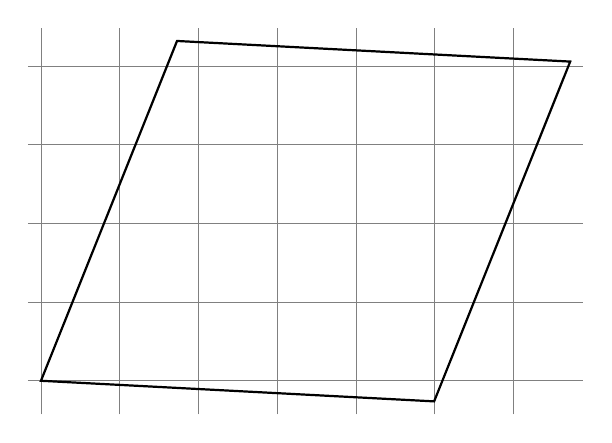
\begin{tikzpicture}[show background grid]
\draw[thick,black,rotate=357] (0,0) -- node{} ++(5.0,0) -- ++(1.5,4.4) -- ++(-5.0,0) --cycle;
\end{tikzpicture}
}
\\\hline
c)&\pbox{5cm}{
Berechne den Flächeninhalt von:\\
\tikzstyle{background grid}=[draw, black!15,step=.5cm]
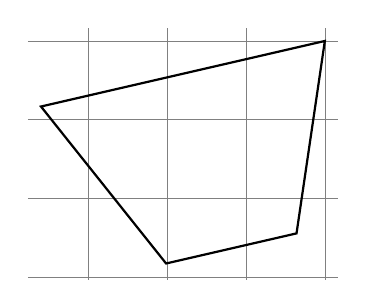
\begin{tikzpicture}[show background grid]
\draw[thick,black,rotate=193] (0,0) -- node[below]{} ++(3.7,0) -- ++(-1.1,2.3) --node[below]{} ++(-1.7,0) --cycle;
\end{tikzpicture}
}
&
d)&\pbox{5cm}{
Berechne den Flächeninhalt von:\\
\tikzstyle{background grid}=[draw, black!15,step=.5cm]
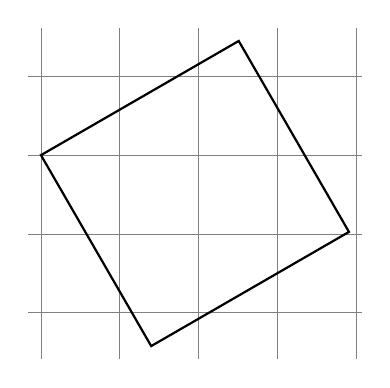
\begin{tikzpicture}[show background grid]
\draw[thick,black,rotate=300] (0,0) -- node[below]{} ++(2.8,0) -- ++(-0.0,2.9) --node[below]{} ++(-2.8,0) --cycle;
\end{tikzpicture}
}
\\\hline
\end{xltabular}
\vspace{0.5cm}
\newpage
\rightline{Datum: 08.12.2023}
\centerline{{\large Lösungen Tägliche Übungen}} 
\vspace{0.5cm}

\begin{xltabular}{\textwidth}{|C{0.75cm}|X|C{0.75cm}|X|}
\arrayrulecolor{black}\hline
a)&\pbox{5cm}{
$\begin{aligned}
geg.: g&=2,6 cm \\
   h&=4,3 cm \\
ges.: A&=? \\
A&=g\cdot h \\
&=2,6\cdot 4,3 \\
\makebox[0pt][l]{\uuline{\phantom{$A=11,18~cm^2$} } }
A&=11,18~cm^2
\end{aligned}$
\tikzstyle{background grid}=[draw, black!15,step=.5cm]
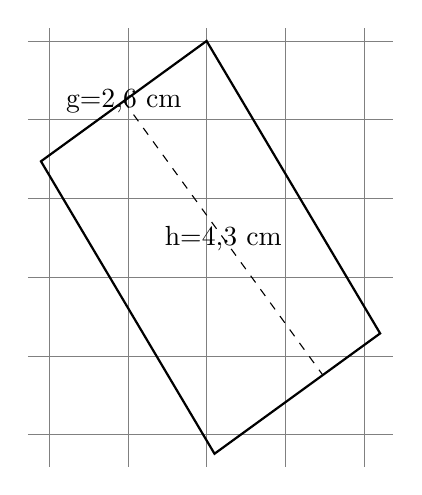
\begin{tikzpicture}[show background grid]
\draw[thick,black,rotate=216] (0,0) -- node{g=2,6 cm} ++(2.6,0) -- ++(0.4,4.3) -- ++(-2.6,0) --cycle;
\draw[dashed,black,rotate=216] (1.3,0)  -- node{h=4,3 cm} ++(0,4.3);
\end{tikzpicture}
}
&
b)&\pbox{5cm}{
$\begin{aligned}
geg.: g&=5 cm \\
   h&=4,4 cm \\
ges.: A&=? \\
A&=g\cdot h \\
&=5\cdot 4,4 \\
\makebox[0pt][l]{\uuline{\phantom{$A=22~cm^2$} } }
A&=22~cm^2
\end{aligned}$
\tikzstyle{background grid}=[draw, black!15,step=.5cm]
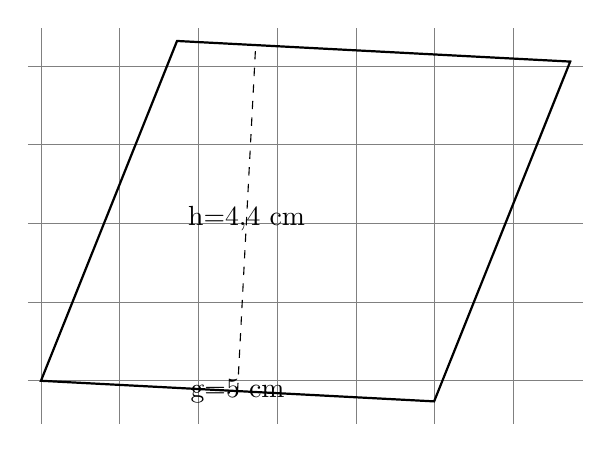
\begin{tikzpicture}[show background grid]
\draw[thick,black,rotate=357] (0,0) -- node{g=5 cm} ++(5.0,0) -- ++(1.5,4.4) -- ++(-5.0,0) --cycle;
\draw[dashed,black,rotate=357] (2.5,0)  -- node{h=4,4 cm} ++(0,4.4);
\end{tikzpicture}
}
\\\hline
c)&\pbox{5cm}{
\tikzstyle{background grid}=[draw, black!15,step=.5cm]
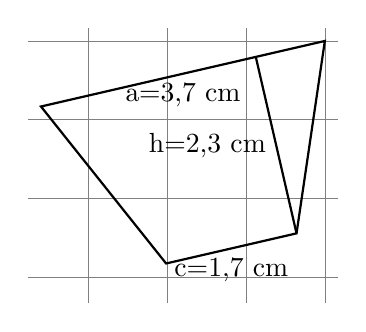
\begin{tikzpicture}[show background grid]
\draw[thick,black,rotate=193] (0,0) -- node[below]{a=3,7 cm} ++(3.7,0) -- ++(-1.1,2.3) --node[below]{c=1,7 cm} ++(-1.7,0) --cycle;
\draw[thick,black,rotate=193] (0.8999999999999999,0) --node[left]{h=2,3 cm}  ++(0,2.3);
\end{tikzpicture}
$\begin{aligned}
geg.: a&=3,7 cm \\
   c&=1,7 cm \\
   h&=2,3 cm \\
ges.: A&=? \\
A&=\frac{a+c}{2}\cdot h \\
&=\frac{3,7+1,7}{2}\cdot2,3\\
\makebox[0pt][l]{\uuline{\phantom{$A=6,21~cm^2$} } }
A&=6,21~cm^2
\end{aligned}$
}
&
d)&\pbox{5cm}{
\tikzstyle{background grid}=[draw, black!15,step=.5cm]
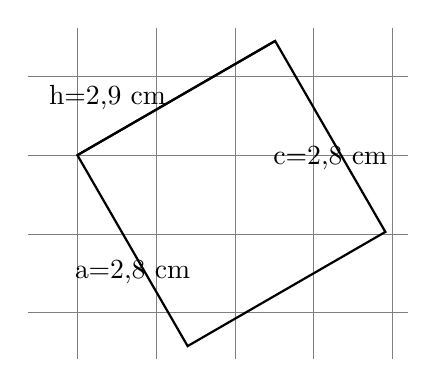
\begin{tikzpicture}[show background grid]
\draw[thick,black,rotate=300] (0,0) -- node[below]{a=2,8 cm} ++(2.8,0) -- ++(-0.0,2.9) --node[below]{c=2,8 cm} ++(-2.8,0) --cycle;
\draw[thick,black,rotate=300] (0.0,0) --node[left]{h=2,9 cm}  ++(0,2.9);
\end{tikzpicture}
$\begin{aligned}
geg.: a&=2,8 cm \\
   c&=2,8 cm \\
   h&=2,9 cm \\
ges.: A&=? \\
A&=\frac{a+c}{2}\cdot h \\
&=\frac{2,8+2,8}{2}\cdot2,9\\
\makebox[0pt][l]{\uuline{\phantom{$A=8,12~cm^2$} } }
A&=8,12~cm^2
\end{aligned}$
}
\\\hline
\end{xltabular}
\vspace{0.5cm}
\end{document}